\section{LHC Search for Higgs Boson}


\begin{frame}{The Standard Model}
\begin{center}
The Standard Model is the compilation of over 100 years of scientific discoveries and is in excellent agreements with a wide range of experimental observations.
\\
\vspace{1em}
\begin{columns}
  \begin{column}{0.5\textwidth}
    \begin{center}
    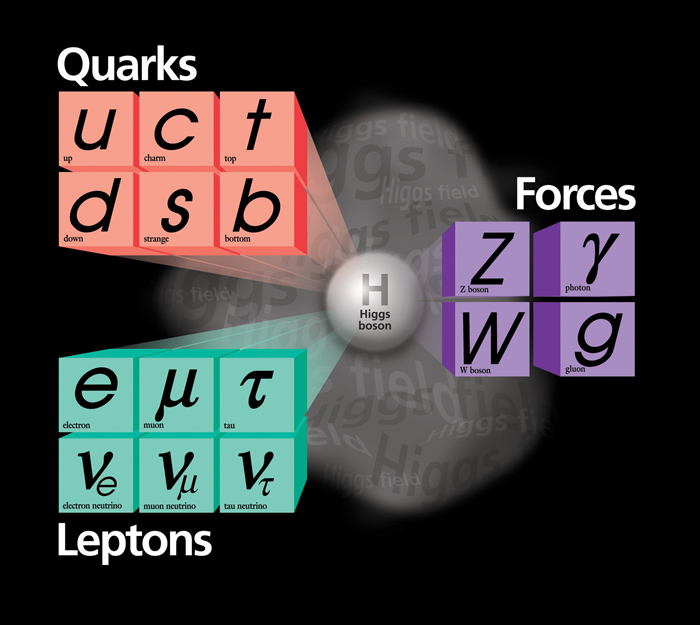
\includegraphics[width=.95\textwidth]{images/standard_model_particles.jpg}\vspace{.1em}
    %\tiny{Source: \url{http://www.fnal.gov/pub/presspass/press_releases/2013/Higgs-Boson-20130314.html}}
    {\fontsize{.1cm}{.001em}\selectfont Source: \url{http://www.fnal.gov/pub/presspass/press_releases/2013/Higgs-Boson-20130314.html}}
    \end{center}
  \end{column}
  \begin{column}{0.5\textwidth}
\begin{center}
\begin{itemize}
  \item
In the Standard Model the simplest solution for the nature of the electroweak symmetry breaking is the introduction of the Higgs field.
\item 
%\vspace{1em}
At the comencement of the LHC the only free parameter of the Standard Model was the Higgs mass.
\end{itemize}
\end{center}
  \end{column}
\end{columns}
\end{center}
\end{frame}

\begin{frame}{Experimental Constraints on the SM Higgs Mass}
\begin{center}
\begin{columns}
      \begin{column}{0.5\textwidth}
        \begin{center}
%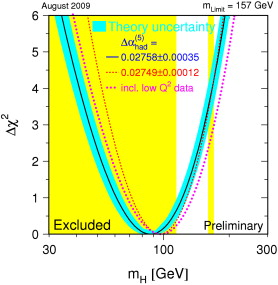
\includegraphics[width=0.99\textwidth]{images/LEPtevatron2009.jpg}
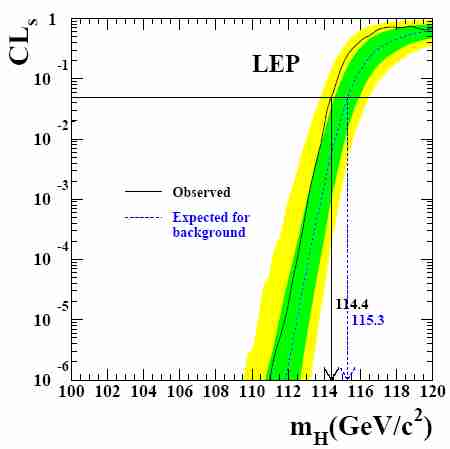
\includegraphics[width=0.65\textwidth]{images/lep2limit.jpg}\\
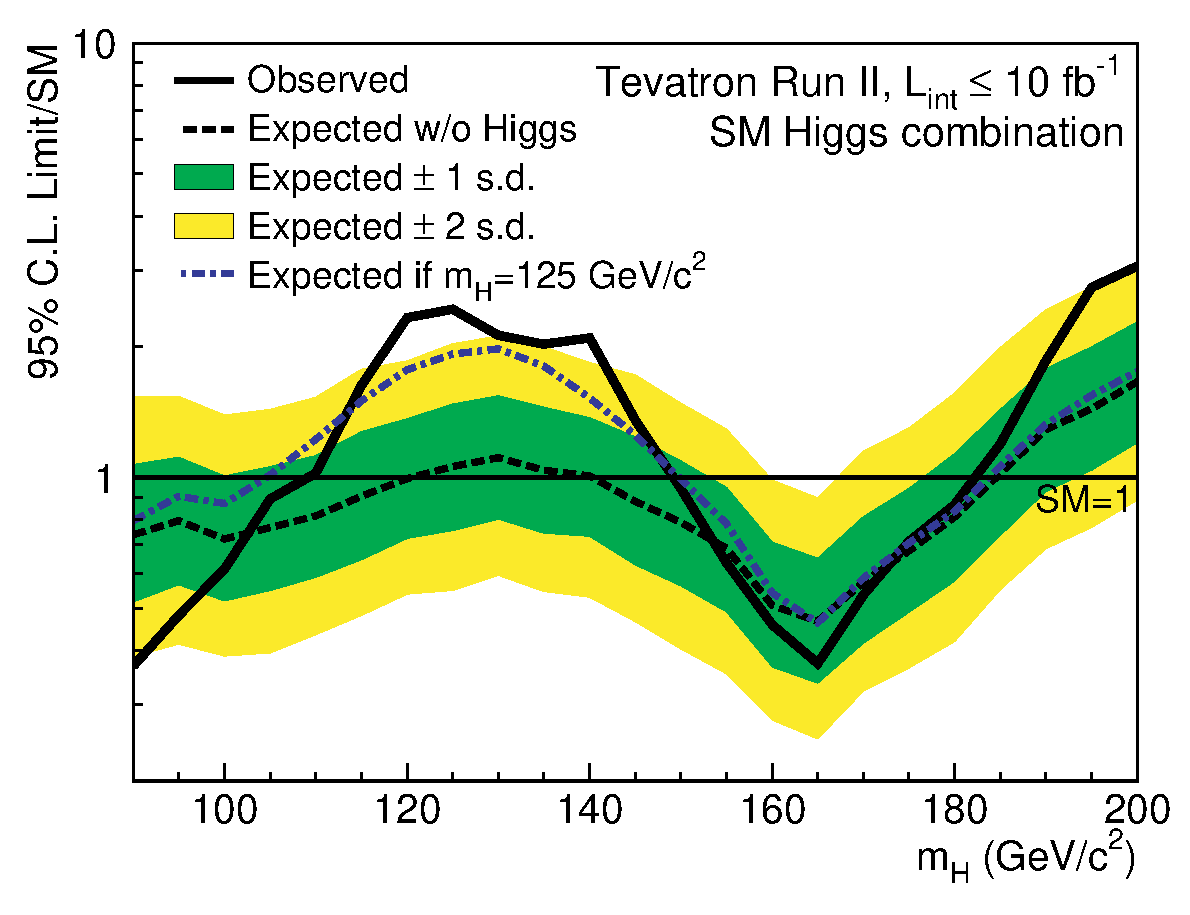
\includegraphics[width=0.75\textwidth]{images/tevsmlimits_feb2013.eps}\\
%\vspace{.001em}
{\fontsize{.1cm}{.001em}\selectfont Source: \url{http://tevnphwg.fnal.gov/}}
\end{center}
\end{column}
\begin{column}{0.5\textwidth}
Experimental constraints:
\begin{itemize}
\item
  LEP excluded with $CL_{95\%}$\\
  \vspace{.5em}
  $m_H$ < 114.4 GeV.\\
  \vspace{1em}
\item
  The latest measurments from Tevetron (July 2013) exclude with $CL_{95\%}$ at:\\
  \vspace{.5em}
  90 GeV < $m_H$ < 109 GeV\\
  149 GeV < $m_H$ < 182 GeV.
\end{itemize}
\end{column}
\end{columns}
\end{center}
\end{frame}

\begin{frame}{Why search for a Higgs at high mass?}
\begin{block}{Discovery}
In 2012 ATLAS and CMS announced the discovery of a new boson at 126 GeV.  In 2013 is was confirmed that this new particle is consistant with a Standard Model Higgs boson.
\end{block}
This analysis is sensative in the 250 to 650 GeV range so why search there?
\begin{itemize}
\item
When we started this analysis in 2011 we didn't know where the Higgs boson would be. (Needed to look everywhere)
\item
Is the new particle THE Standard Model Higgs boson.
\item
Are there other Higgs bosons?
\end{itemize}
\footnotesize
\begin{block}{Beyond the Standard Model}
Many Beyond the Standard Model (BSM) theories extend the simple Higgs sector of the Standard Model and lead to more complicated particle spectrum. Very often one of the new particles has properties very similar to the Standard Model Higgs.
\end{block}
\end{frame}





%\begin{frame}{The Higgs Mechanism}
%\begin{center}
%  \begin{itemize}
%  \item
%    A simple solution for the nature of the electroweak symmetry breaking is introducing the Higgs field.
%  \item
%    The Higgs field is also the means by which elementary particles acquire mass.
%  \item
%    The Higgs boson is the smallest possible excitation of the Higgs field.
%  \item
%    The Higgs mass is a free parameter.
%  \end{itemize}
%\end{center}
%\end{frame}


%\begin{frame}{Particle Accelerators}
%\begin{center}
%Particle accelerators accelerate particles to high energies.
%\begin{columns}
%  \begin{column}{0.4\textwidth}
%This allows us to:
%    \begin{itemize}
%    \item
%      Look deeper into matter (E $\propto \dfrac{1}{size}$ ). ``microscope''
%    \item
%      Discover new heavier particles ($E = mc^{2}$).
%    \item
%      Probe early conditions of the Universe (E = kT).
%    \end{itemize}
%  \end{column}
%  \begin{column}{0.6\textwidth}
%    \begin{center}
%    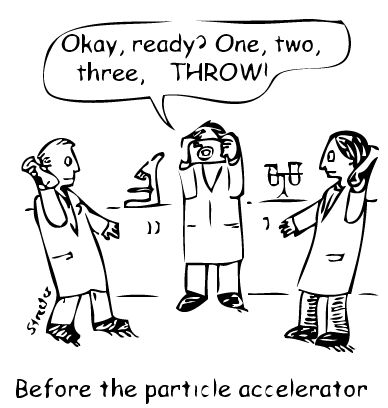
\includegraphics[width=0.79\textwidth]{images/before_accelerators.png}
%    \end{center}
%  \end{column}
%\end{columns}
%All this while being controlled in the laboratory.
%\end{center}
%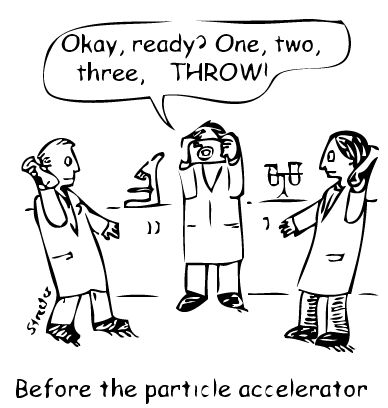
\includegraphics[width=0.99\textwidth]{images/before_accelerators.png}
%\end{frame}


%\begin{frame}{LHC}
%\begin{center}
%Four Experiments
%\begin{itemize}
%\item
%  CMS - General Purpose
%\item
%  ATLAS - General Purpose
%\item
%  LHCb - b-physics
%\item
%  ALICE - heavy ion
%\end{itemize}
%\vspace{.5em}
%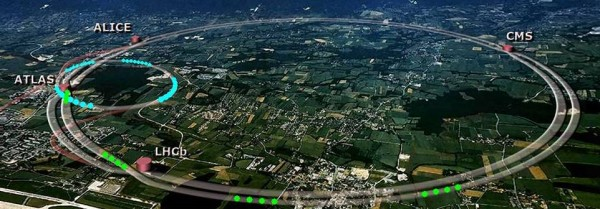
\includegraphics[width=0.99\textwidth]{images/lhc-sim-600x209.jpg}
%\end{center}
%\end{frame}



%\begin{frame}{The LHC Accelerator}
%  \begin{center}
%    \begin{itemize}
%    \item
%      Proton-proton collider
%    \item
%      Circumference: 26.7 km
%    \item
%      Tunnel: 100 meters underground
%    \item
%      dipoles operate at 8.3 T
%    \item
%      1232 superconducting Niobium-Titanium magnets
%    \item
%      better vacuum and colder than inter-planetary  space
%    \end{itemize}
  
%\vspace{.5em}
%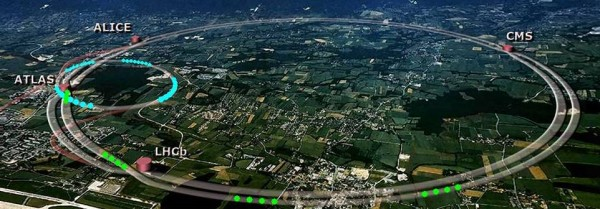
\includegraphics[width=0.99\textwidth]{images/lhc-sim-600x209.jpg}

%  \end{center}
%\end{frame}





%\begin{frame}{Injection Scheme}
%\begin{center}
%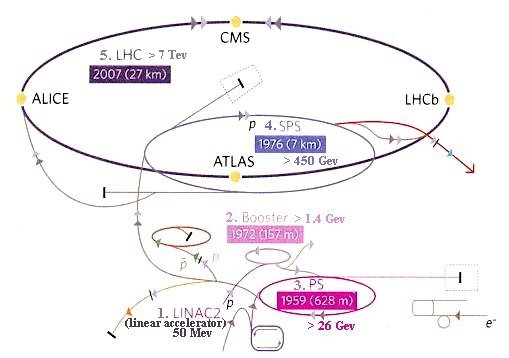
\includegraphics[width=0.49\textwidth]{images/lhc_schematic.jpg}
%\begin{itemize}
%\item
%Linac2 $\rightarrow$ 50 MeV
%\item
%Proton Synchrotron  $\rightarrow$ 1.4 GeV
%\item
%Super Protron Synchrotron  $\rightarrow$ 450 GeV
%\item
%LHC  $\rightarrow$ 4.0 TeV
%\end{itemize}
%\end{center}
%\end{frame}


\begin{frame}{LHC Environment}
%\begin{center}
\begin{columns}
\begin{column}{0.5\textwidth}
\begin{center}
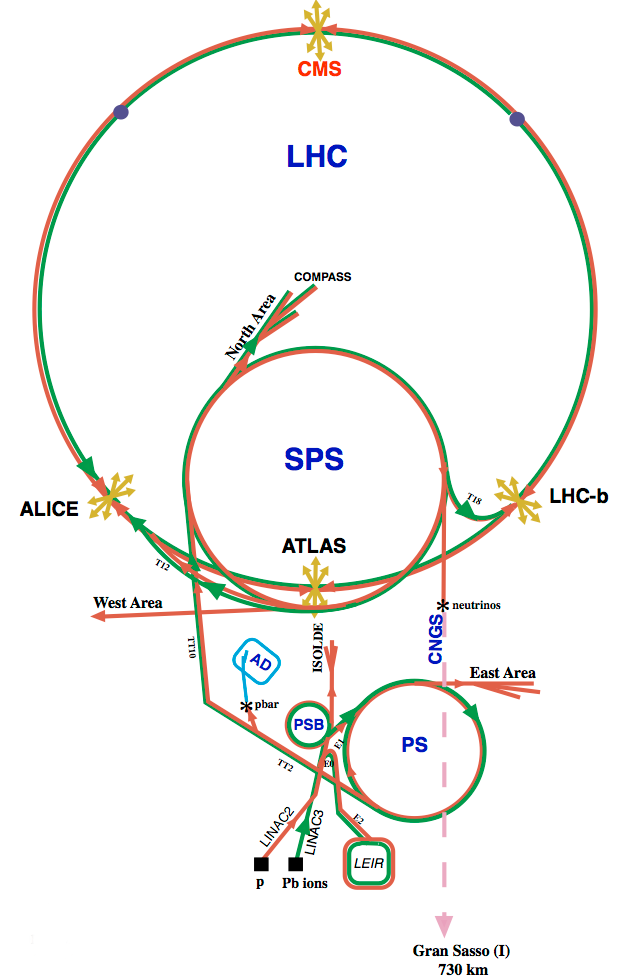
\includegraphics[width=0.79\textwidth]{images/cern-acc.png}\\
{\fontsize{.1cm}{.001em}\selectfont Source: \url{http://www.quantumdiaries.org/2011/10/24/the-25-ns-pumpkin-teeth/}}
\end{center}
\end{column}
\begin{column}{0.5\textwidth}
\begin{center}
In 2012 $\sqrt{s}$ = 8 TeV\\
\vspace{.8em}
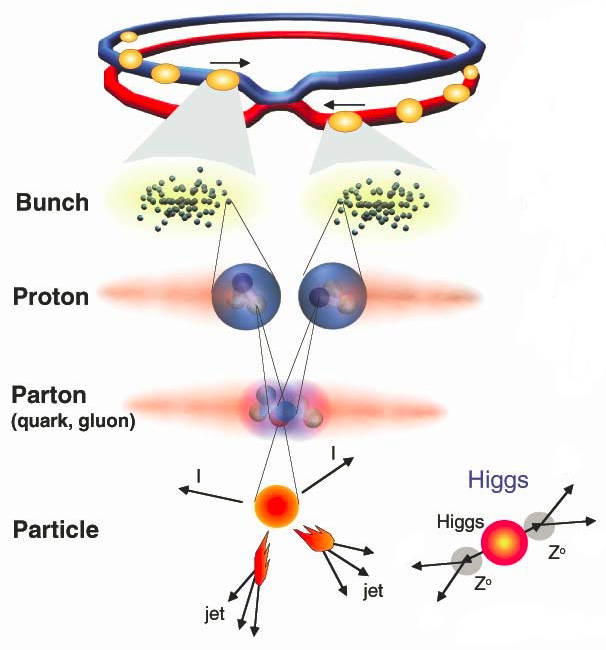
\includegraphics[width=0.89\textwidth]{images/HKrT0L.png}\\
{\fontsize{.1cm}{.001em}\selectfont Source: \url{Haijun Yang, Colloquium Shanghai Jian Tong University, Sept 12, 2012}}
\end{center}
\end{column}
\end{columns}
%
%HKrT0L.png
%\end{center}
\end{frame}


\begin{frame}{LHC Delivered Data}

\begin{columns}
\begin{column}{0.5\textwidth}
\begin{center}
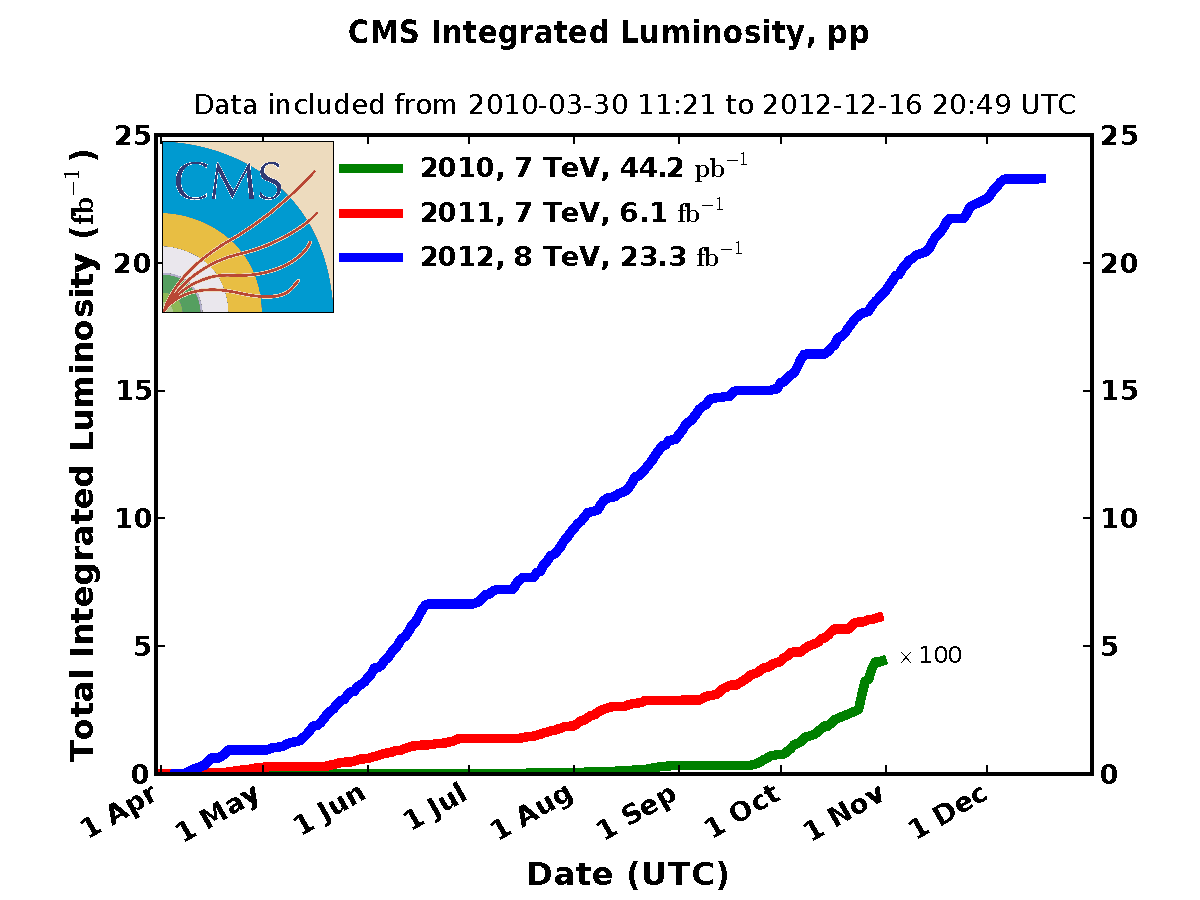
\includegraphics[width=0.85\textwidth]{images/int_lumi_cumulative_pp_2.pdf}\\
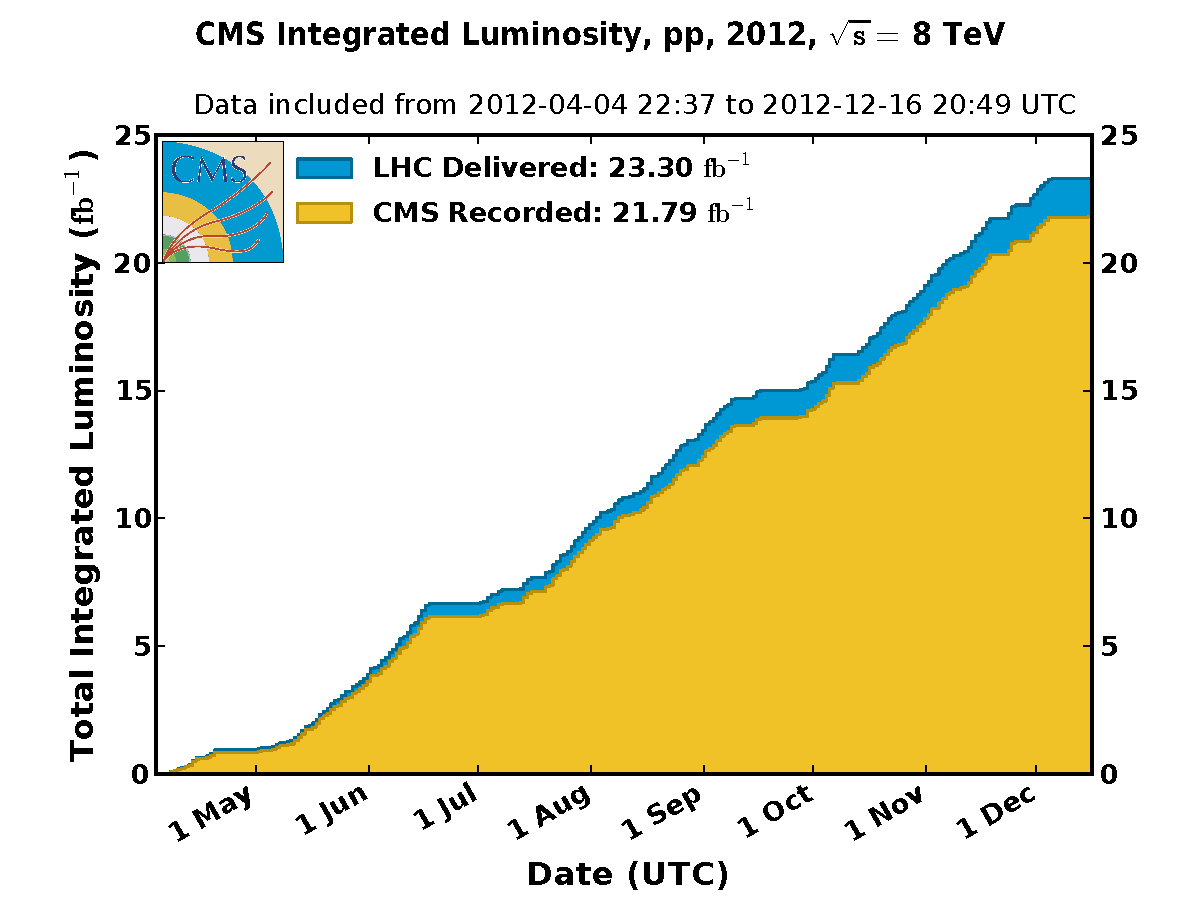
\includegraphics[width=0.85\textwidth]{images/int_lumi_per_day_cumulative_pp_2012.pdf}\\
\end{center}
\end{column}
\begin{column}{0.5\textwidth}
\begin{itemize}
\item
CMS has done extremely well during Run I (2010-2012).
\item
Data-taking efficiency was very high (95\%)
\item
Main challenge of the 2012 was how to deal with pileup.
\end{itemize}
\begin{center}
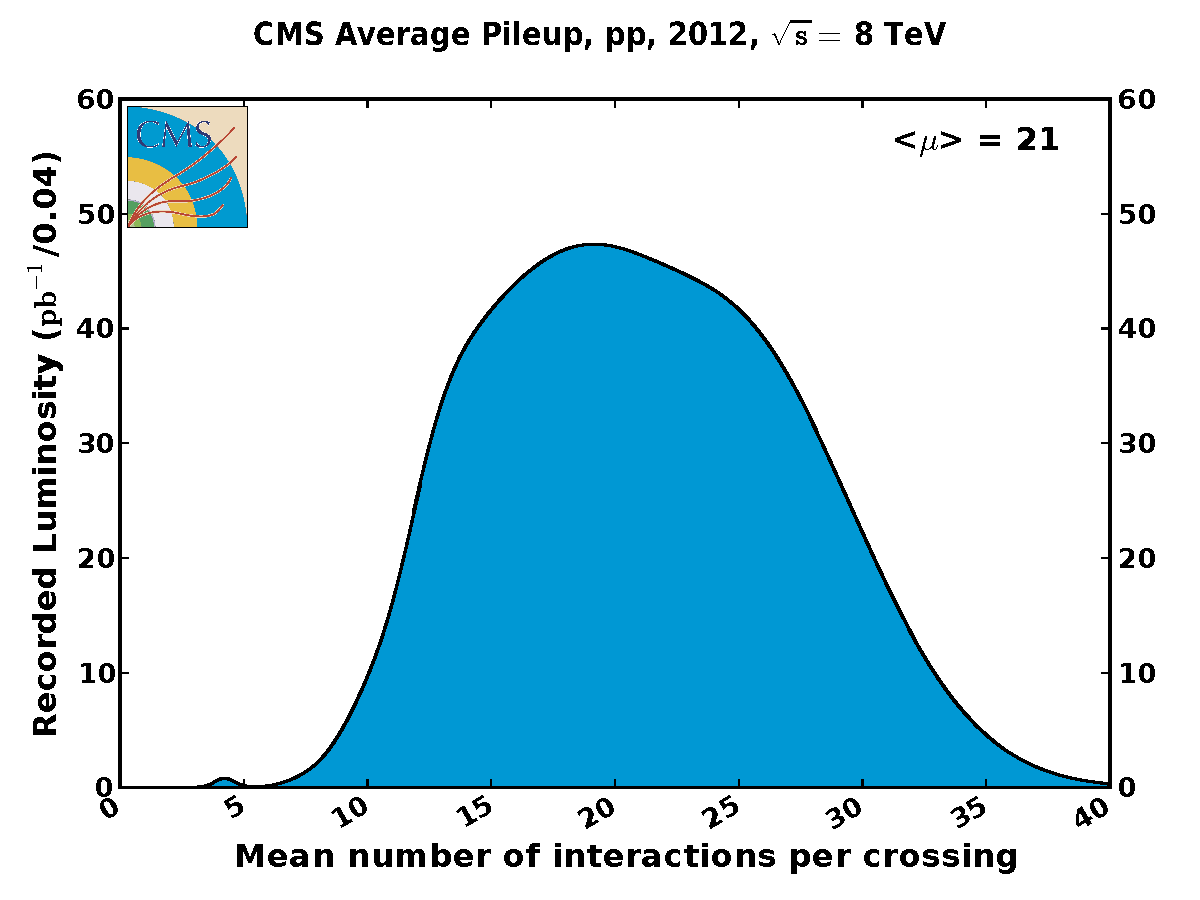
\includegraphics[width=0.85\textwidth]{images/pileup_pp_2012.pdf}
{\fontsize{.1cm}{.001em}\selectfont Source: \url{http://twiki.cern.ch/twiki/bin/view/CMSPublic/LumiPublicResults}}
\end{center}
\end{column}
\end{columns}

%\begin{center}
%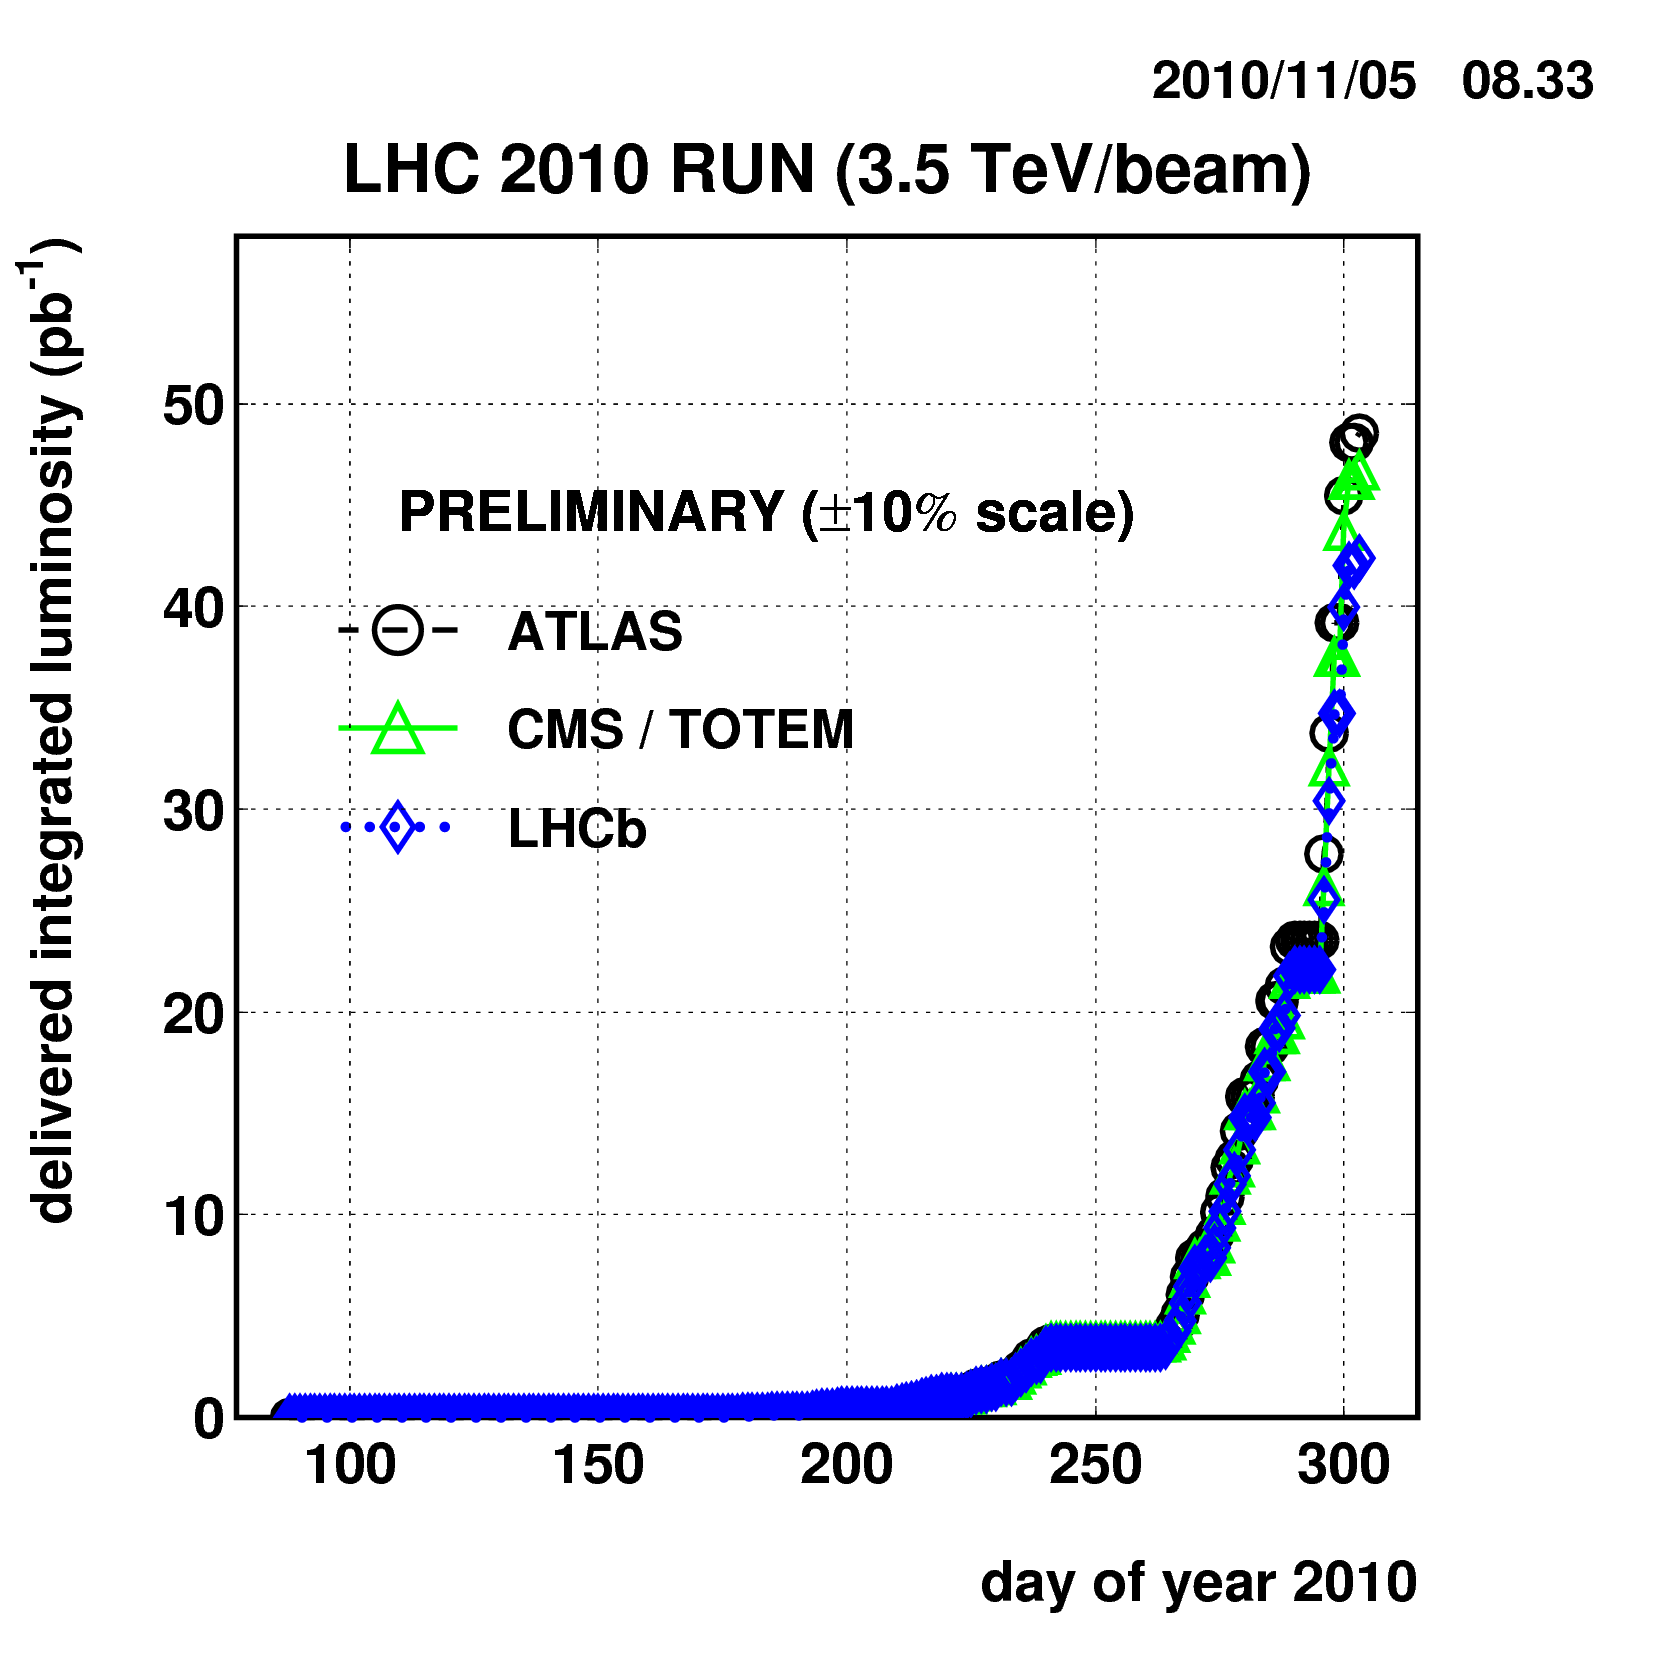
\includegraphics[width=0.33\textwidth]{images/2010_lhc_luminocity.png}
%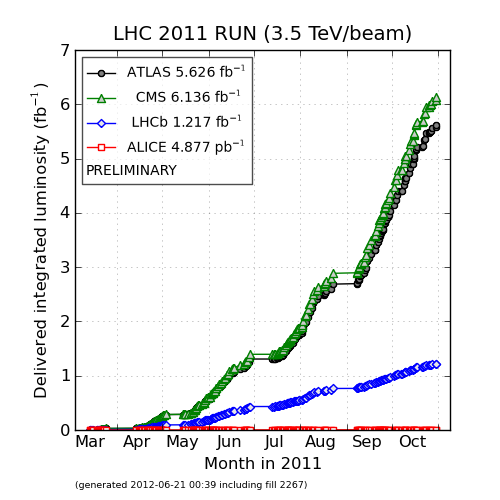
\includegraphics[width=0.33\textwidth]{images/2011_lhc_luminocity.png}
%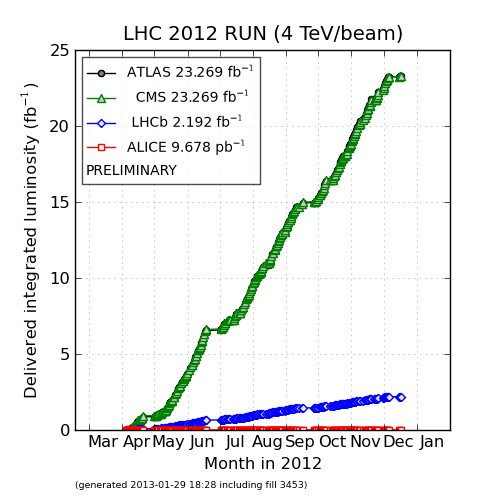
\includegraphics[width=0.33\textwidth]{images/2012_lhc_luminocity.png}
%\end{center}
\end{frame}

\begin{frame}{Compact Muon Solenoid}
\begin{center}
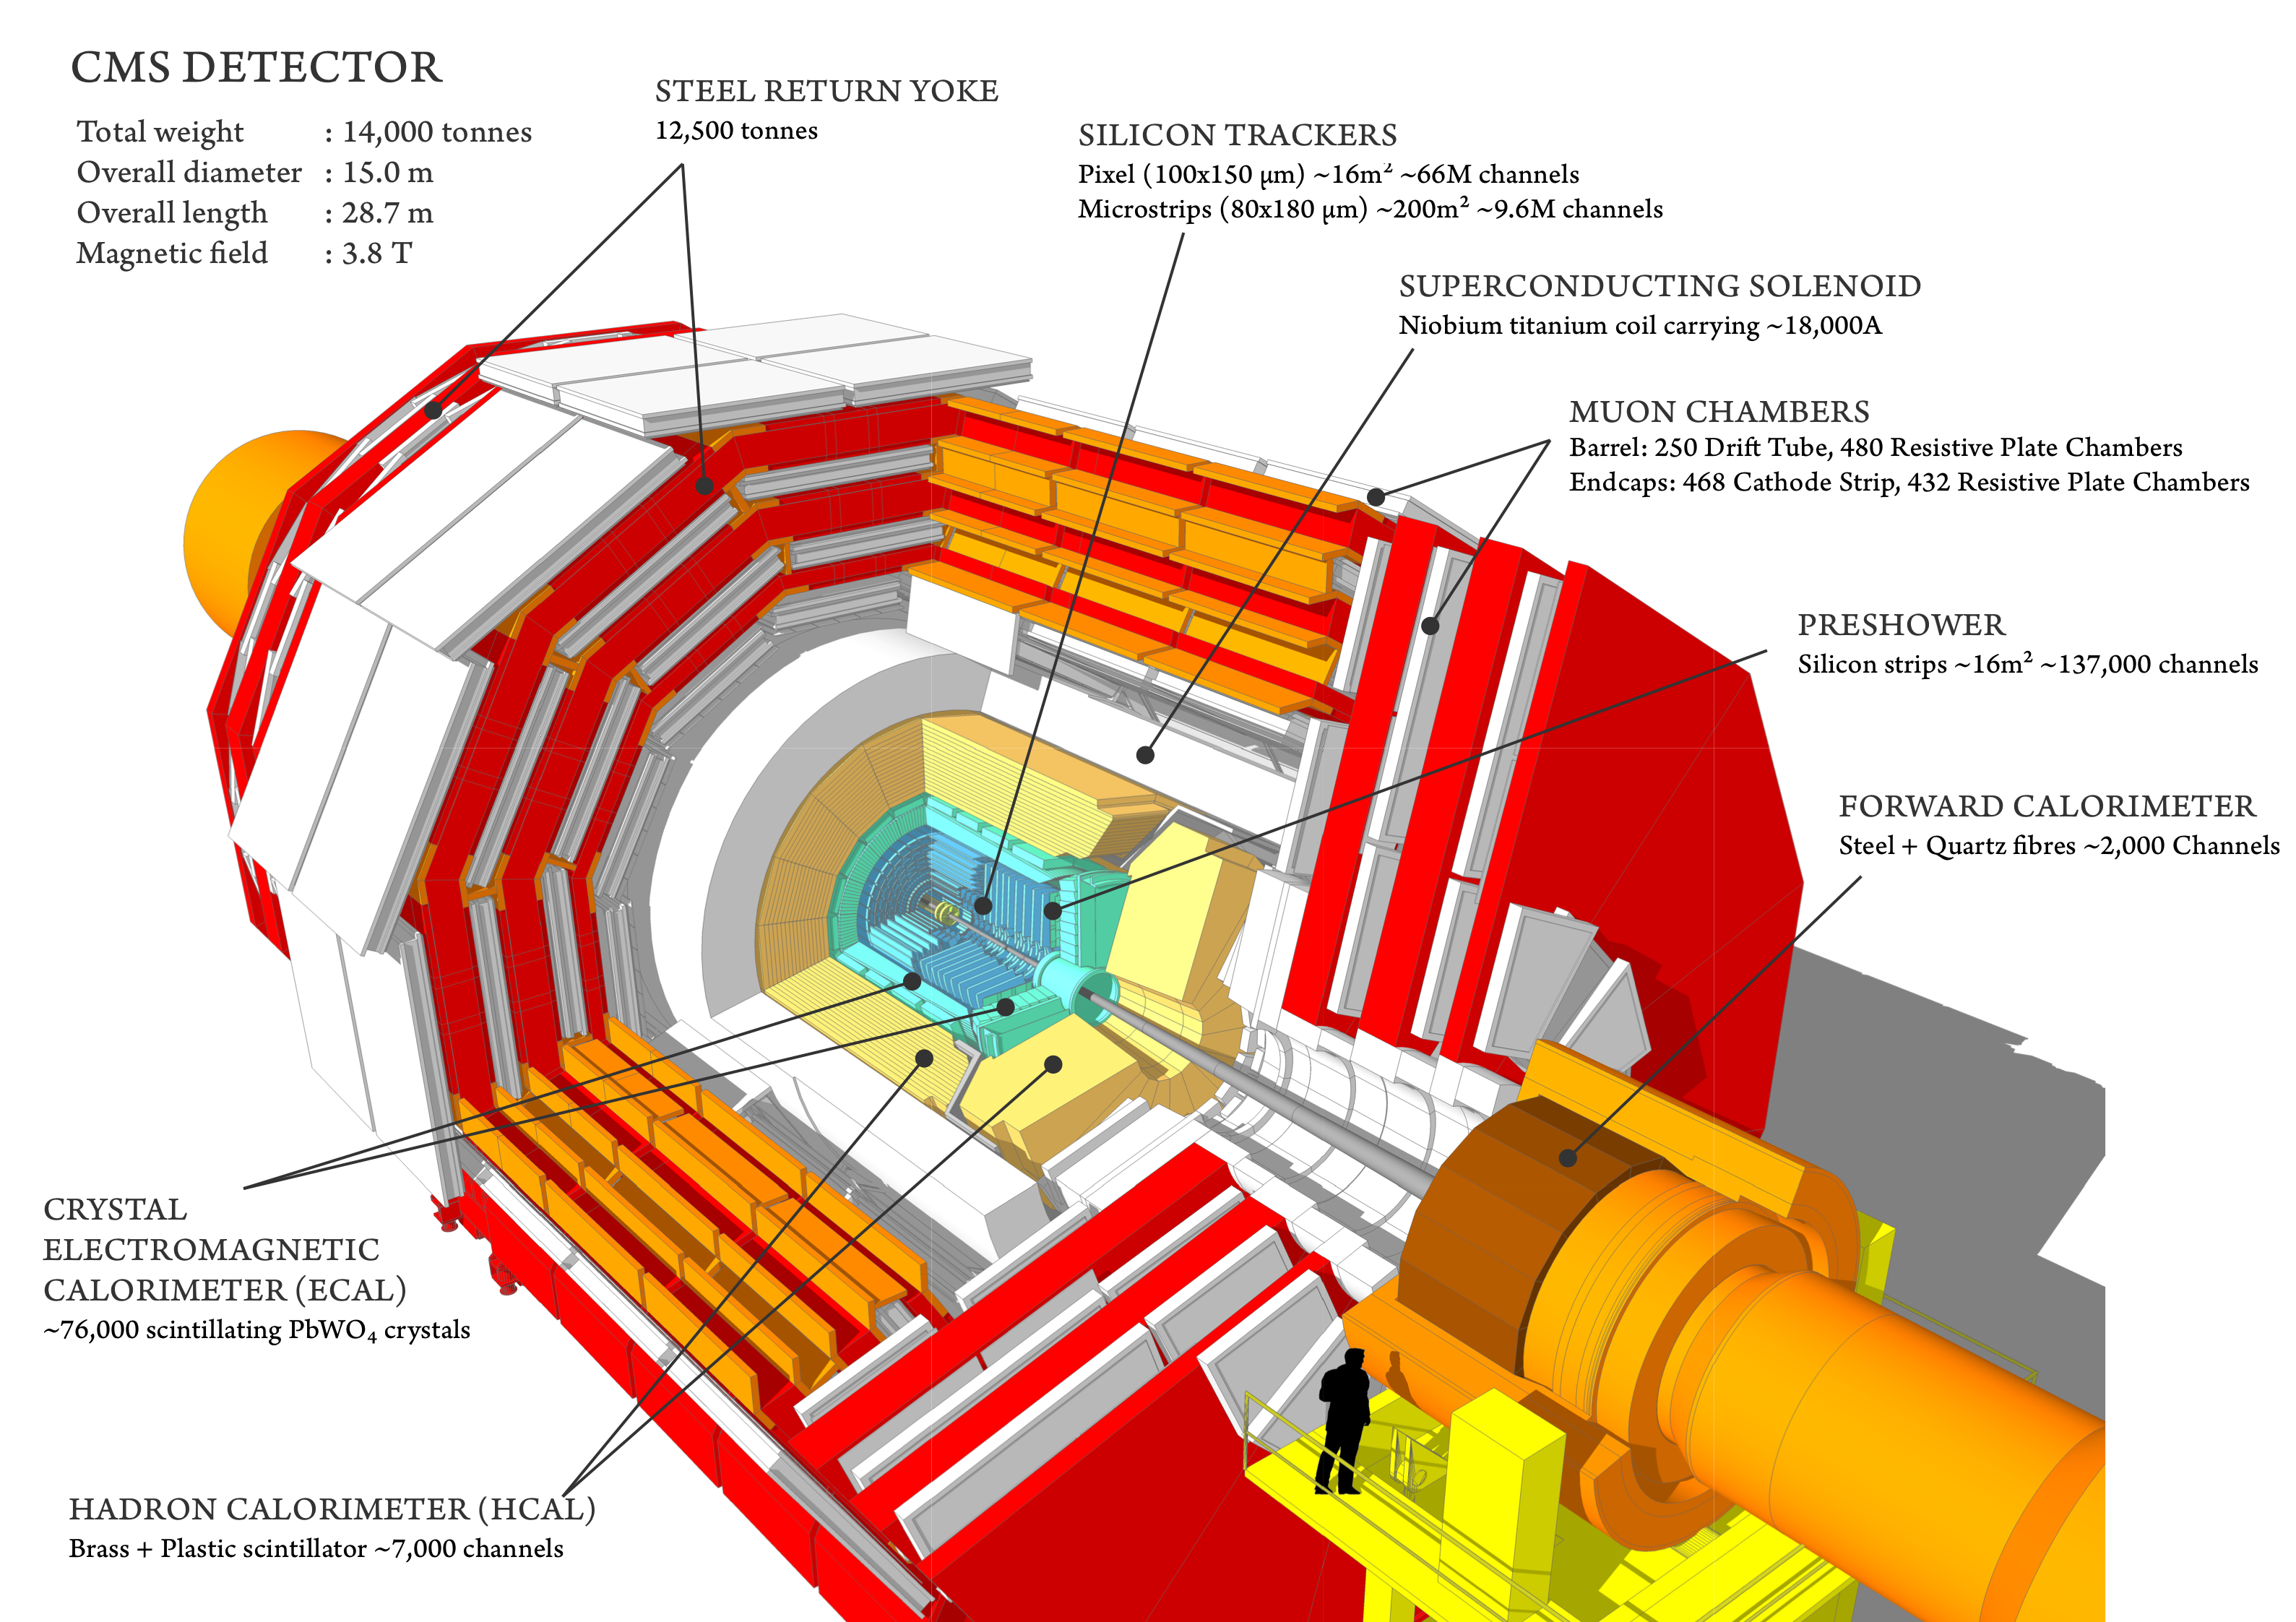
\includegraphics[width=0.85\textwidth]{images/cms_120918_03.png}\\
{\fontsize{.1cm}{.001em}\selectfont Source: \url{http://www.fnal.gov/pub/presspass/press_releases/2013/Higgs-Boson-20130314.html}}
%/CMScollaborationPoster.png}

\end{center}
\end{frame}


\begin{frame}{CMS Slice}
\begin{center}
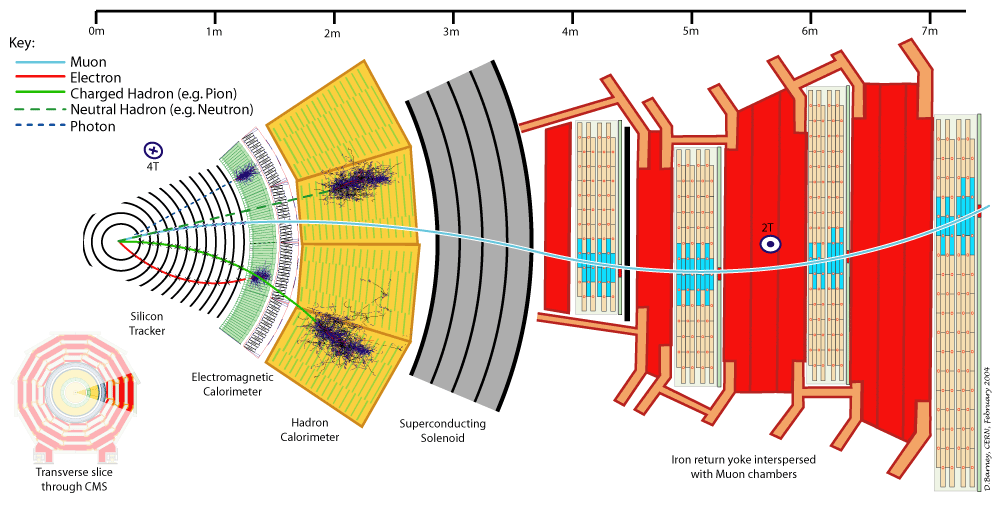
\includegraphics[width=0.99\textwidth]{images/CMS_Slice.png}
\end{center}
\end{frame}

\begin{frame}{CMS Detector Glossary}
\begin{center}
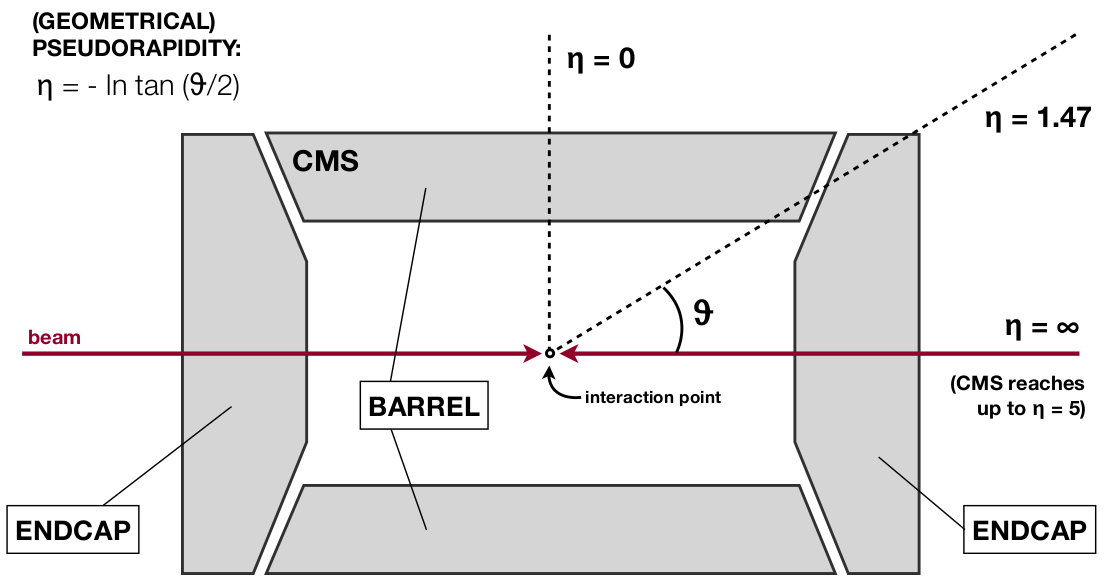
\includegraphics[width=0.99\textwidth]{images/DetectorGlossary.png}
\end{center}
\end{frame}

%\begin{frame}{Space Holder}
%\begin{center}
%\end{center}
%\end{frame}

\begin{frame}{Higgs Production}
\begin{center}
\begin{columns}
  \begin{column}{0.35\textwidth}
    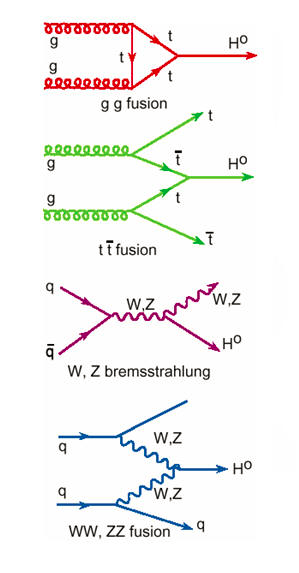
\includegraphics[width=0.99\textwidth]{images/higgs_production_feynman.png}
  \end{column}
  \begin{column}{0.65\textwidth}
    Gluon-gluon fusion ($gg \rightarrow H$) and vector-boson fusion ($qq \rightarrow qqH$) are dominant
    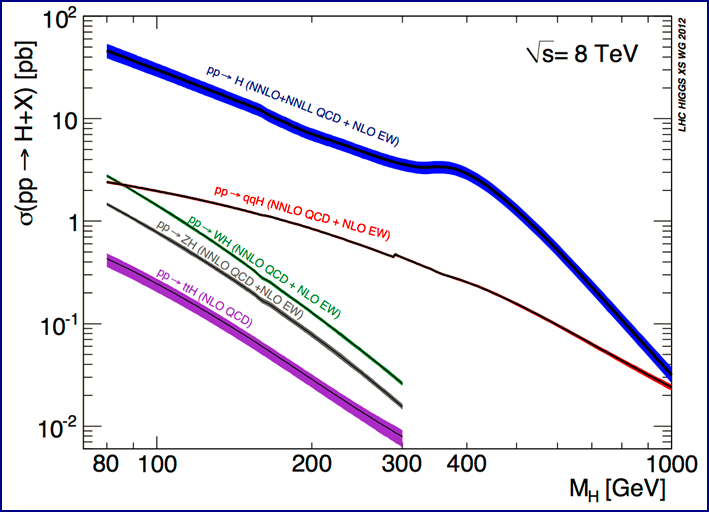
\includegraphics[width=0.99\textwidth]{images/higgs_production_lhc.png}
  \end{column}
\end{columns}
\end{center}
\end{frame}








\begin{frame}{Higgs Decay}
\begin{center}
\begin{columns}
  \begin{column}{0.5\textwidth}
    \begin{itemize}
      \item
        Discovery strategy depends on the available decay channels.
      \item
        Decays with leptons provide clean signatures.
    \end{itemize}
  \end{column}
  \begin{column}{0.5\textwidth}
    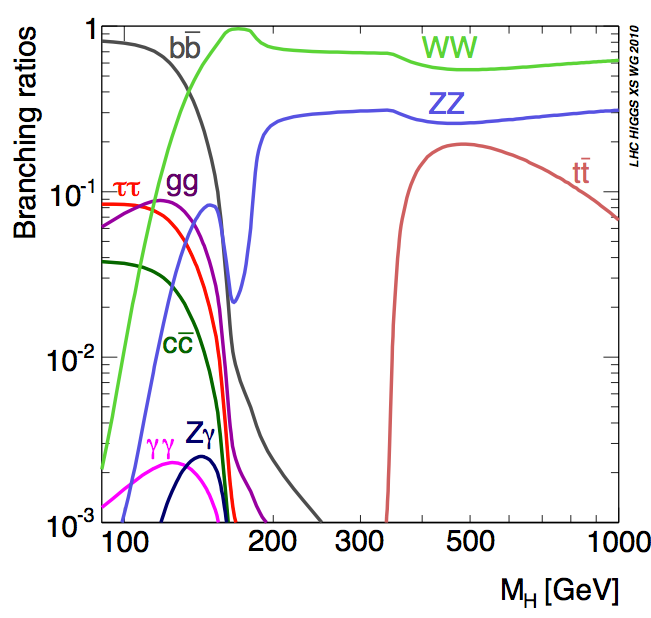
\includegraphics[width=0.99\textwidth]{images/branching_ratio.png}
  \end{column}
\end{columns}
Main Discovery Channels
\begin{itemize}
\item
  $H \rightarrow \gamma \gamma$
\item
  $H \rightarrow W^+W^-$
\item
  $H \rightarrow ZZ$
\end{itemize}
\end{center}
\end{frame}





\begin{frame}{The Heavy Higgs Decay}
\begin{center}
  For a heavy ($m_H$ > 200 GeV) Higgs boson the Higgs decays predominantly to vector boson pairs.
\\  The fully leptonic decay modes are:\\
\vspace{.5em}
$H \rightarrow WW \rightarrow \Plp \Pgn \Plm \Pagn$\\
$H \rightarrow ZZ \rightarrow \Plp \Plm \Plp \Plm$\\
$(\Pl = \Pe , \Pgm)$\\
\vspace{1em}
$H \rightarrow ZZ \rightarrow \Plp \Plm \Plp \Plm$ (The ``golden'' Channel)\\
\end{center}

Pros:
\footnotesize
\begin{itemize}
\item
  Decay chain can be fully reconstructed.
\item
  High precision lepton measurements gives a narrow invariant mass peak.
\end{itemize}
\vspace{1em}
\small
Cons:
\footnotesize
\begin{itemize}
  \item
    The branching ratio of $Z \rightarrow \Plp \Plm$ is only 3.37\% so less than 0.5\% of the $H \rightarrow ZZ$ events will end up in the ``golden'' channel.
\end{itemize}


%\begin{itemize}
%  \item

%    Decay to two Z bosons is the most promising discovery channel for $m_H > 180 GeV$.
%  \item
%    If both Z bosons decay to electrons or muons you get a very clean signature.
%\end{itemize}
%    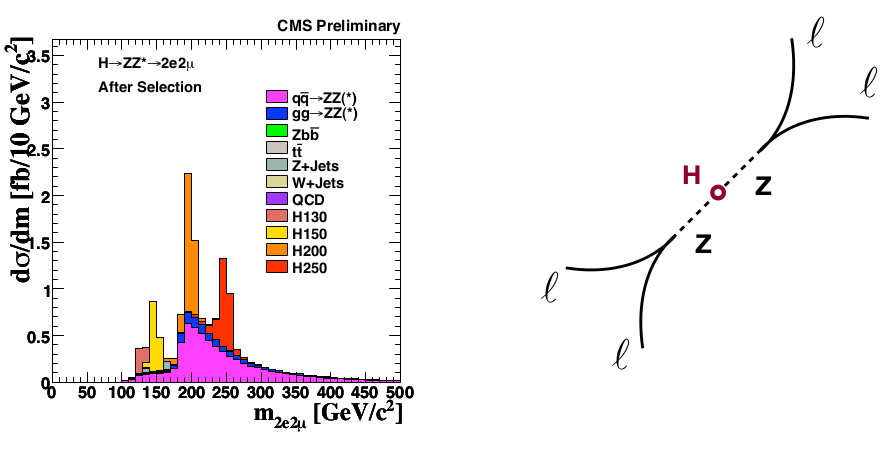
\includegraphics[width=0.99\textwidth]{images/ZZdecay.png}
%\begin{columns}
%  \begin{column}{0.5\textwidth}
%  \end{column}
%  \begin{column}{0.5\textwidth}
%  \end{column}
%\end{columns}

\end{frame}

\begin{frame}{The $H \rightarrow ZZ \rightarrow llqq$ Channel}
\begin{center}

 When a Z decays to quarks they hadronize and form ``jets.'' These are complex objects and challenging to reconstruct. 

    If we allow one Z to decay leptonicly and the other to quarks we get.\\
    \vspace{.5em}
    $H \rightarrow ZZ \rightarrow \Plp \Plm \Pq \Paq$\\
    $(q = u,d,c,s,b)$
\begin{columns}
  \begin{column}{0.7\textwidth}
     Pros:\footnotesize
     \begin{itemize}
     \item
     Large branching ratios
     \begin{itemize}
     \item
       BR($Z \rightarrow qq$) = 70\%
     \item
       BR($ZZ \rightarrow 2l2q$) = $\color{red}{20} \color{black} \times BR(ZZ \rightarrow 4l)$
     \end{itemize}
   \item
     Fully decay is reconstructed (closed kinematics)
     \end{itemize}
     \vspace{1em}
     \small
     Cons:\footnotesize
     \begin{itemize}
     \item
       Resolution of jet momentum reconstruction is worse than for leptons.
     \item
       Large background coming from Z production in conjunction with QCD jets ($\sim 10^5$ > signal).
     \end{itemize}
  \end{column}
  \begin{column}{0.3\textwidth}
    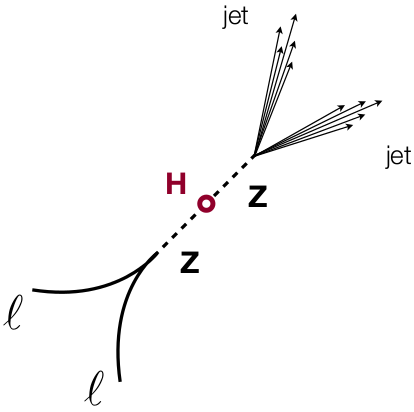
\includegraphics[width=0.99\textwidth]{images/h_zz_2l2q.png}
  \end{column}
\end{columns}

\end{center}
\end{frame}


%\begin{frame}{Traditional Jet Approach: Caloremeter Jets}
%\end{frame}



\begin{frame}{Traditional Jet Approach: Caloremeter Jets}
For CaloJets we assume most particles will reach the calorimeters close to each other.  So all we have to do is cluster the energy deposits in the calorimeter.

\begin{columns}[T]
  \begin{column}{0.6\textwidth}
    \vspace{2em}
    \begin{column}{0.5\textwidth}
      Pros:
      \begin{itemize}
      \item
        straightforward
      \item
        fast and unaffected by event complexity
      \end{itemize}
    \end{column}
    \begin{column}{0.5\textwidth}
      Cons:
      \begin{itemize}
      \item
        response is $p_{T}$-dependent
      \item
        lose low $p_{T}$ charged particles
      \item
        HCAL resolution
      \end{itemize}
    \end{column}
  \end{column}
  \begin{column}{0.40\textwidth}
    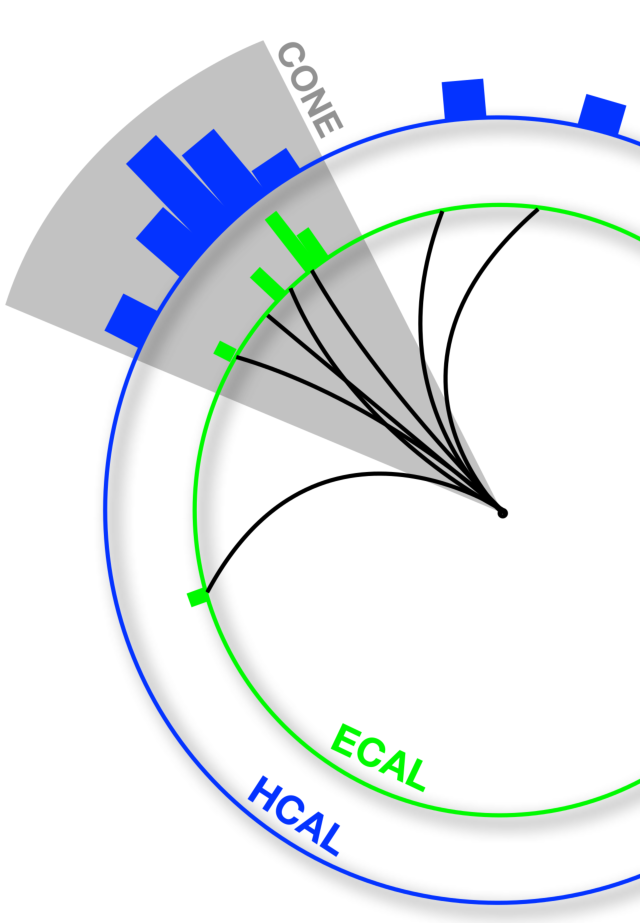
\includegraphics[width=0.99\textwidth]{images/calojets.pdf}
  \end{column}
\end{columns}
\end{frame}


\begin{frame}{Particle Flow}
The particle flow algorithm attempts to reconstruct all stable final state particles using all of the CMS sub-detectors.

\begin{columns}[T]
  \begin{column}{0.6\textwidth}
\footnotesize
    \begin{itemize}
    \item
      1. Get tracks linked to a single ECAL cluster if electron ID says OK create an electron.
    \end{itemize}
  \end{column}
  \begin{column}{0.40\textwidth}
    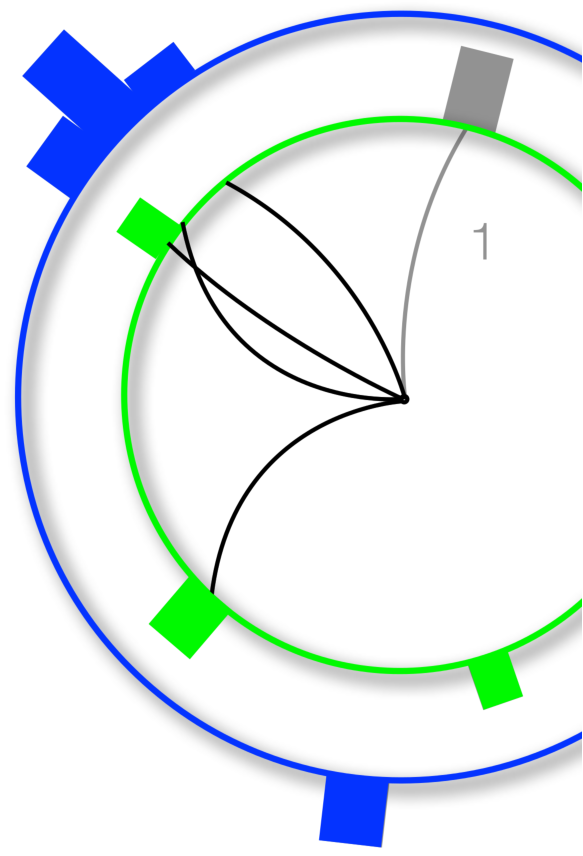
\includegraphics[width=0.99\textwidth]{images/pf1.pdf}
  \end{column}
\end{columns}
\end{frame}



\begin{frame}{Particle Flow}
The particle flow algorithm attempts to reconstruct all stable final state particles using all of the CMS sub-detectors.

\begin{columns}[T]
  \begin{column}{0.6\textwidth}
\footnotesize
    \begin{itemize}
\footnotesize
    \item
      1. Get tracks linked to a single ECAL cluster if electron ID says OK create an electron.
    \item
      2. If not then if there are compatible hits in muon chambers create a muon if not create a charged hadron.
    \end{itemize}
  \end{column}
  \begin{column}{0.40\textwidth}
    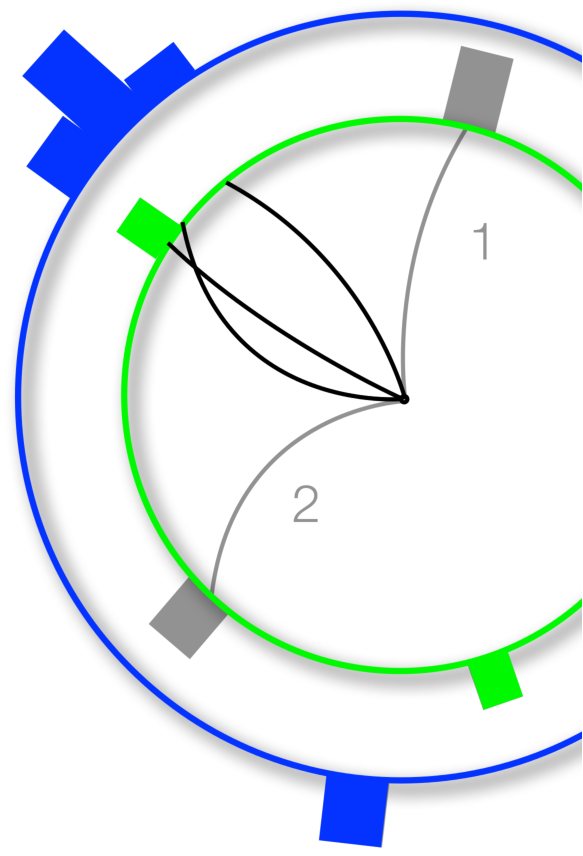
\includegraphics[width=0.99\textwidth]{images/pf2.pdf}
  \end{column}
\end{columns}
\end{frame}


\begin{frame}{Particle Flow}
The particle flow algorithm attempts to reconstruct all stable final state particles using all of the CMS sub-detectors.

\begin{columns}[T]
  \begin{column}{0.6\textwidth}
\footnotesize
    \begin{itemize}
\footnotesize
    \item
      1. Get tracks linked to a single ECAL cluster if electron ID says OK create an electron.
    \item
      2. If not then if there are compatible hits in muon chambers create a muon if not create a charged hadron.
    \item
      3. For each HCAL cluster get all the linked tracks and all ECAL clusters linked to tracks. If the energy in the calorimeters is compatible with the tracks then create a charged hadron for each track.  If the energy is greater than the tracks create photons or neutral hadrons equal to the missing calorimeter energy.
    \end{itemize}
  \end{column}
  \begin{column}{0.40\textwidth}
    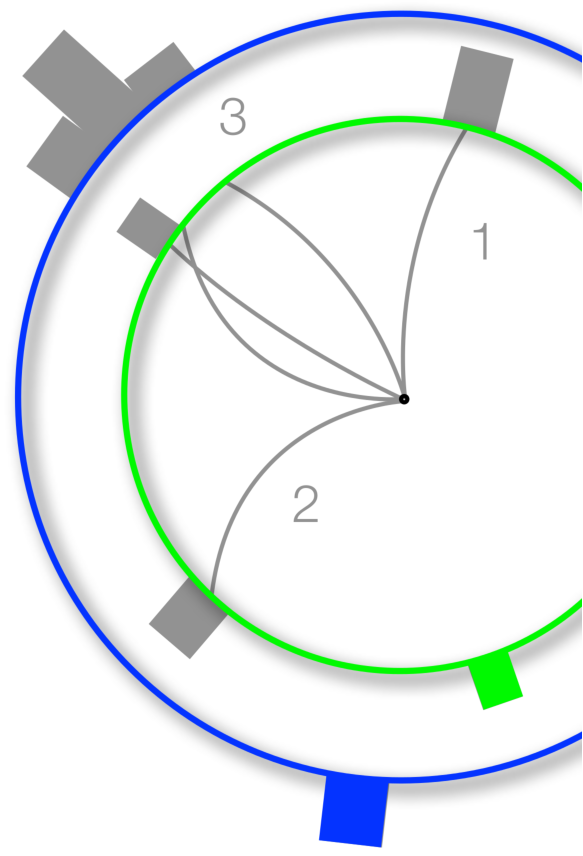
\includegraphics[width=0.99\textwidth]{images/pf3.pdf}
  \end{column}
\end{columns}
\end{frame}

\begin{frame}{Particle Flow}
The particle flow algorithm attempts to reconstruct all stable final state particles using all of the CMS sub-detectors.

\begin{columns}[T]
  \begin{column}{0.6\textwidth}
    \begin{itemize}
      \footnotesize
    \item
      1. Get tracks linked to a single ECAL cluster if electron ID says OK create an electron.
    \item
      2. If not then if there are compatible hits in muon chambers create a muon if not create a charged hadron.
    \item
      3. For each HCAL cluster get all the linked tracks and all ECAL clusters linked to tracks. If the energy in the calorimeters is compatible with the tracks then create a charged hadron for each track.  If the energy is greater than the tracks create photons or neutral hadrons equal to the missing calorimeter energy.
    \item
      4. For the remaining ECAL (HCAL) clusters that are not linked to tracks create a photon (neutral hadron).
    \end{itemize}
  \end{column}
  \begin{column}{0.40\textwidth}
    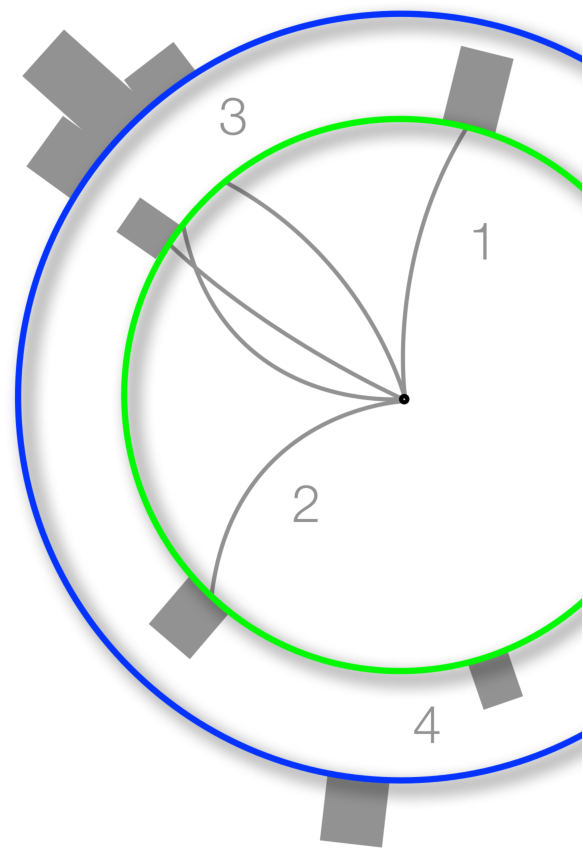
\includegraphics[width=0.99\textwidth]{images/pf4.pdf}
  \end{column}
\end{columns}
\end{frame}


%\begin{frame}{Discovering the Higgs}
%\begin{center}
%\begin{columns}
%  \begin{column}{0.5\textwidth}
%  \end{column}
%  \begin{column}{0.5\textwidth}
%  \end{column}
%\end{columns}
%\end{center}
%\end{frame}
